\section{Measurements}
\label{sec:2}


The measurements were performed on Nov. 7th 2024 at 12:00h with assistance from and in the office of Dr. Frédéric Boone. 
The instrument was controlled via a local machine interface, using instructions provided online \cite{user_instr}. 
Due to delays accumulated from previous groups, we were not able to perform step 1 of the aforementioned work items and were instructed to use the pre-existing calibration to save time.

We took measurements of four different targets, \textit{Sagittarius A*}, \textit{RC cloud \TODO{What is this actually? Do we need to explain?}}, \textit{Cygnus X1} and \textit{Cassiopeia A}. 
The coordinates were already pre-defined in the antenna control interface.
The positions of the antenna during each measurement were recorded through a webcam on top of the roof and can be seen below in \autoref{fig:antenna positions}. 


\begin{figure}[H]
    \centering
    \subfloat[Sagittarius A]
    {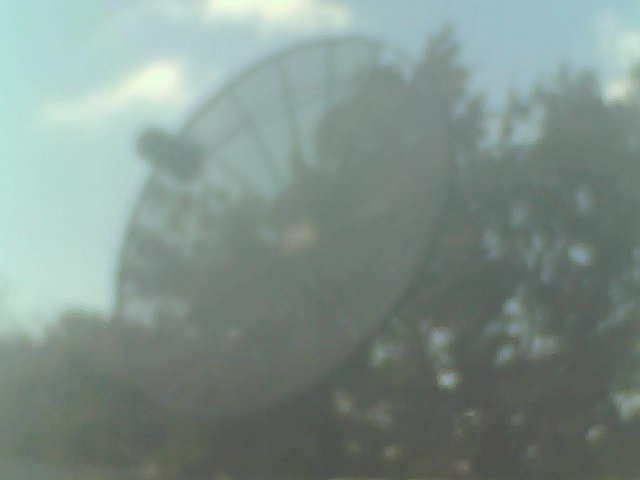
\includegraphics[width=0.45\textwidth]{Doc/Graphics/Antenna position - SagittA.jpg}
    \label{fig:SagA}}
    \subfloat[RC cloud]
    {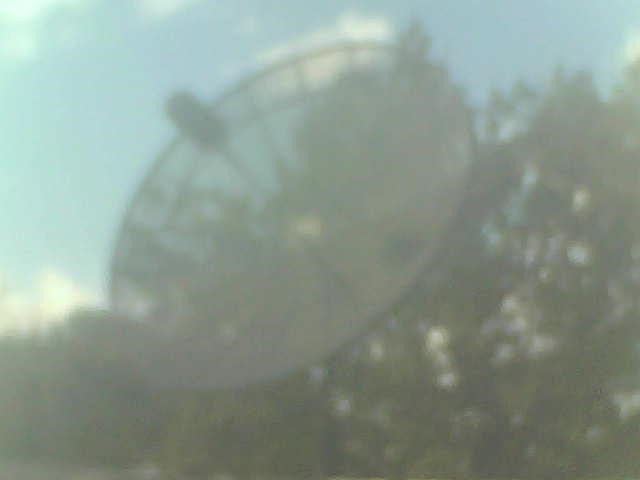
\includegraphics[width=0.45\textwidth]{Doc/Graphics/Antenna position - RC cloud.jpg}
    \label{fig:RC}}

    \subfloat[Cygnus X1]
    {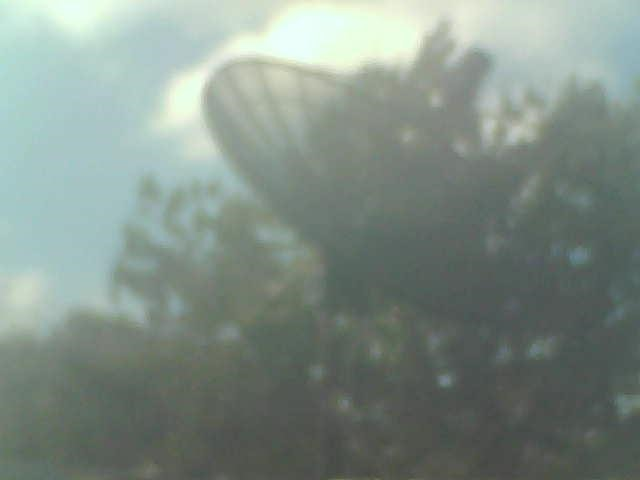
\includegraphics[width=0.45\textwidth]{Doc/Graphics/Antenna position - Cyg.jpg}
    \label{fig:Cyg}}
    \subfloat[Cassiopeia A]
    {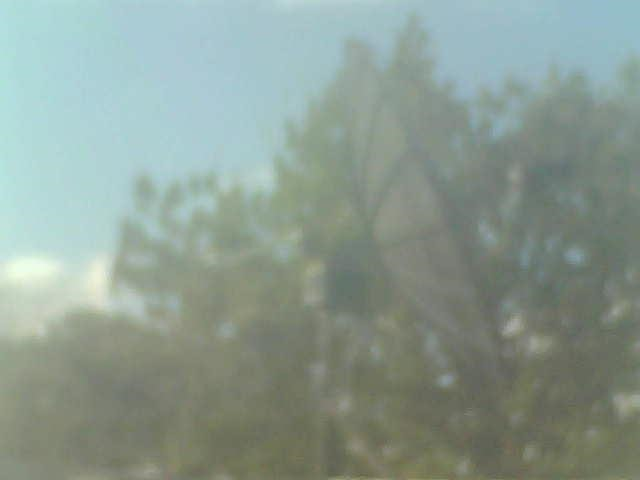
\includegraphics[width=0.45\textwidth]{Doc/Graphics/Antenna position - Cass.jpg}
    \label{fig:fCass}}
    
    \caption{Antenna positions during all four measurements}
    \label{fig:antenna positions}
\end{figure}


\newpage
Each measurement was timed for a duration of \SIrange{36}{40}{\second}, resulting in 3 - 4 JSON datasets per target. Each dataset represents measured average power for a series of frequency steps between \SIrange{1419.8}{1421.0}{\mega\hertz}. Since we had multiple datasets per target, we first calculated the average of those for each target. The resulting datasets can be seen in \autoref{fig:2-original-measurements}.

\begin{figure}[H]
    \centering
    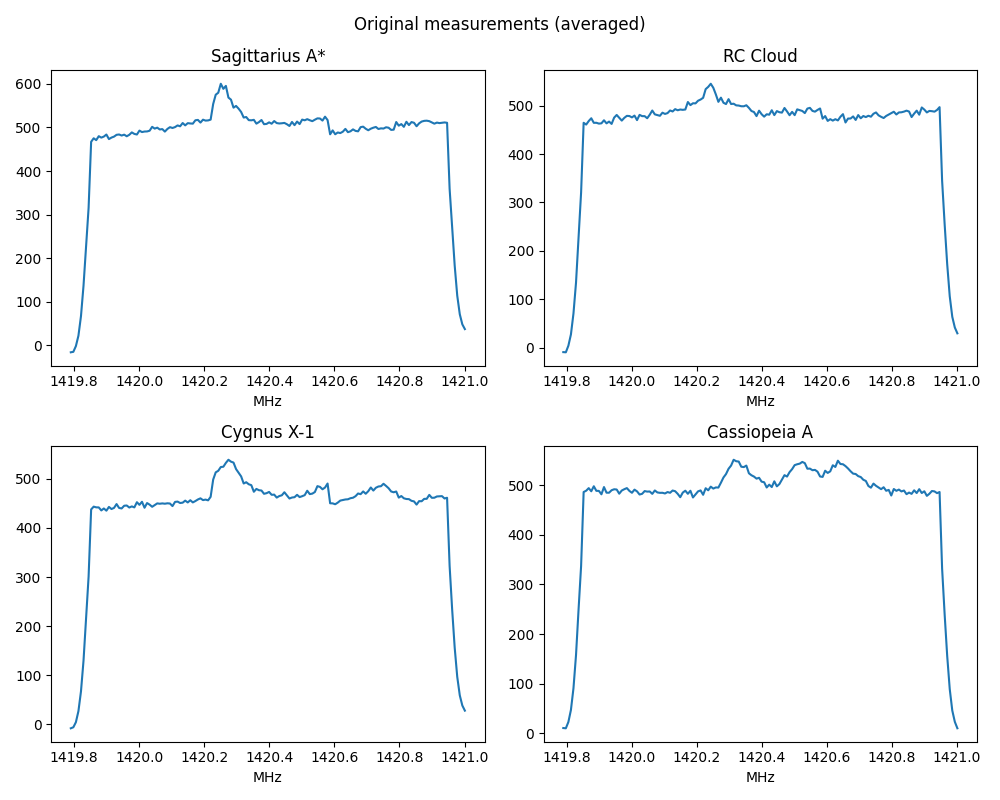
\includegraphics[width=\linewidth]{Doc//Graphics/2-original-measurements.png}
    \caption{Original, averaged measurements per target}
    \label{fig:2-original-measurements}
\end{figure}

\vspace{1cm}
Now, we only care about the 21cm hydrogen line at \SI{1420.4}{\mega\hertz}. To remove the baseline power visible over the whole bandwidth, we fitted a line over the baseline and subtracted it from the measurements. We also clipped the data to disregard the frequencies on the edges of the bandwidth. In \autoref{fig:2-cleaned-measurements}, the hydrogen line is clearly visible, albeit a bit offset from the expected \SI{1420.4}{\mega\hertz} due to Doppler shift.

\begin{figure}[H]
    \centering
    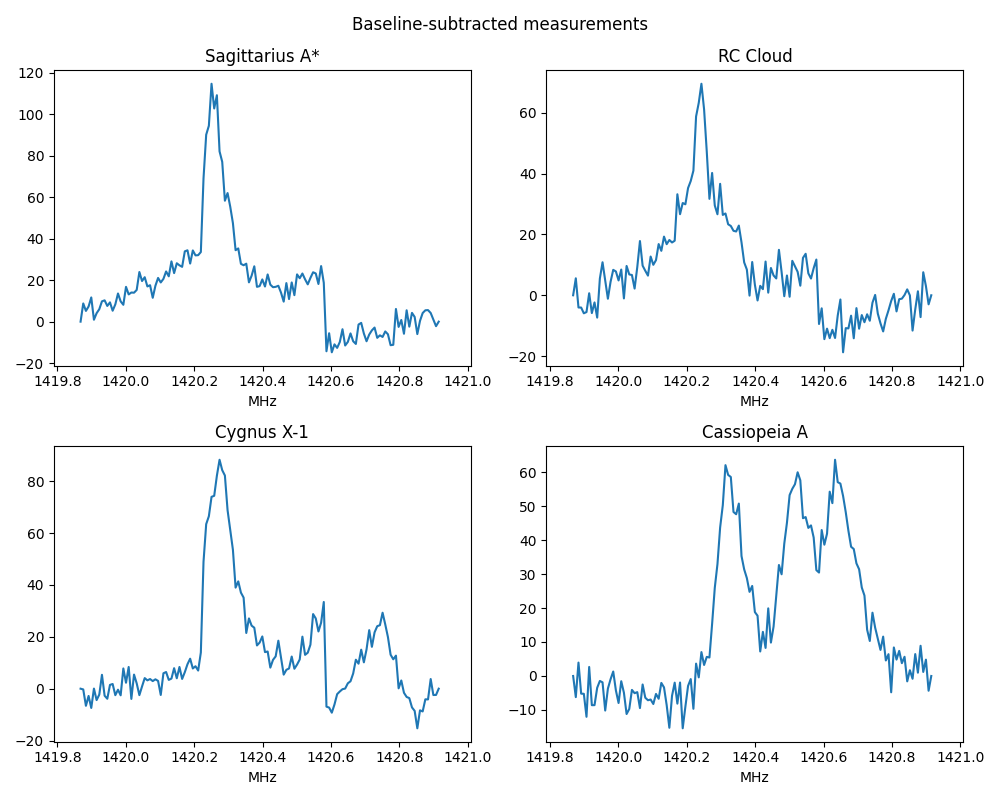
\includegraphics[width=1\linewidth]{Doc//Graphics/2-cleaned-measurements.png}
    \caption{Baseline-subtracted measurements with edges clipped}
    \label{fig:2-cleaned-measurements}
\end{figure}

\vspace{1cm}
The measurements are in antenna units, with 1 antenna unit corresponding to 790 Janskys. Furthermore, we convert Janskys into SI-units, with 1 Jansky corresponding to \SI{e-26}{\watt\per\square\meter\per\hertz}. The resulting power per area per frequency can be seen in \autoref{fig:2-si-measurements}. We will analyze this data in \autoref{sec:3} to calculate the number density of hydrogen in our galaxy.

\begin{figure}[H]
    \centering
    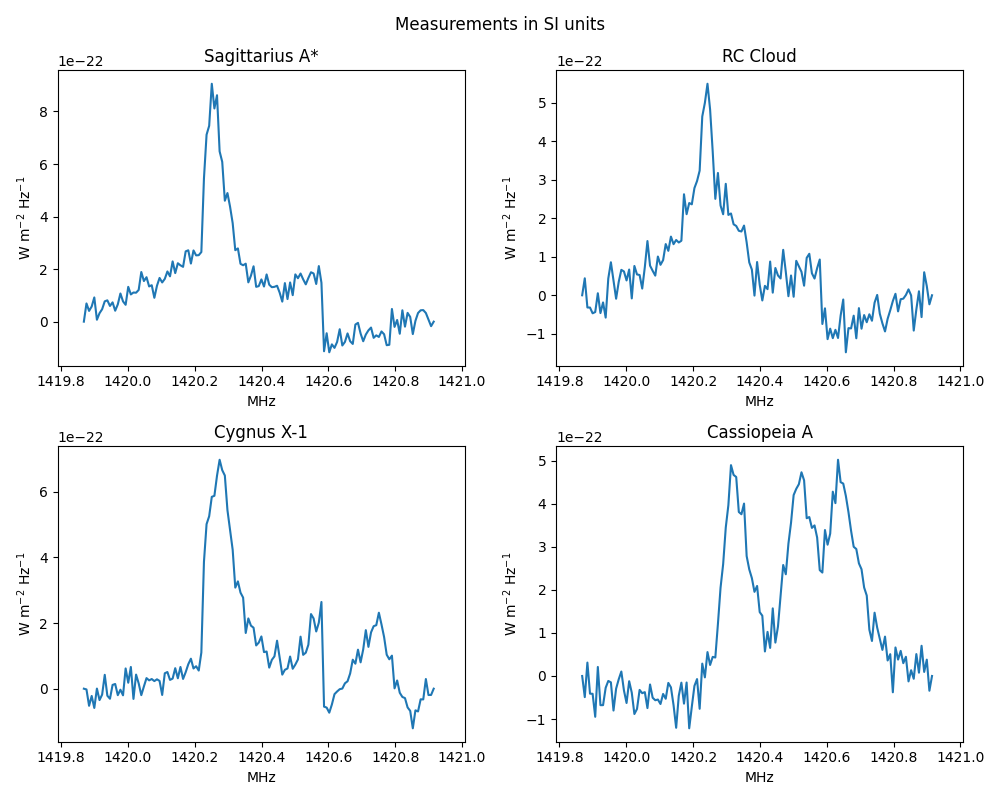
\includegraphics[width=1\linewidth]{Doc//Graphics/2-si-measurements.png}
    \caption{Measurements in SI units}
    \label{fig:2-si-measurements}
\end{figure}